\section{Topic Models}\label{sec:plate_notation}
In this section, topic models that are explored in the experiment are detailed.
This covers the standard \gls{lda} from \citet{blei2003latent}, our category and author metadata models, which build on the concept of \gls{lda}, and our taxonomy metadata model, which uses the \acrlong{pam}.

\subsection{Standard \gls{lda}}
The purpose of \gls{lda}, and topic models in general, is to create a tool for exploring collections of text.
Topic models do this by uncovering the underlying semantic structure of a text collection by using hierarchical Bayesian models.
\Gls{lda} uncovers this semantic structure by discovering patterns of word use in documents and finding topics based on these~\cite{blei2009topic}.

The standard \gls{lda} by \citet{blei2003latent} imagines the following generative process:
$D$ is the number of documents in the corpus, $N_d$ is the number of words in document $d$, $V$ is the size of the vocabulary, and $K$ is the number of topics.
Topics are represented as distributions over words and documents are represented as distributions of topics.
\Gls{lda} assumes that the topics are shared across the corpus, while the document-topic distributions are unique for each document.

For each topic $k \in \{1,\dots, K\}$ a topic-word distribution $\beta_k$ is sampled from a V-dimensional Dirichlet distribution parameterized by $\eta$.
That is, K topics $\beta_{1:k}$ are sampled, each being a distribution over the vocabulary, written as: $\beta_k \sim Dirichlet(\eta)$.
Likewise, for each document $d \in \{1,\dots, D\}$ a document-topic distribution $\theta_d$ is sampled from a K-dimensional Dirichlet distribution parameterized by $\alpha$.
For each word $n \in \{1, \dots, N_d\}$ in each document $d$, a topic $z_{d,n}$ is sampled from a K-multinomial distribution $\theta_d$, and then a word $w_{d,n}$ is sampled from a V-multinomial distribution $\beta_{z_{d,n}}$.
The generative process for each document is seen in these steps:

\vspace{\topsep}
\begin{enumerate}
	\item Draw topic proportion $\theta_d \sim Dirichlet(\alpha)$
	\item For each word $n$ in the document:
	\begin{enumerate}
		\item Draw topic assignment $z_{d,n} \sim Mult(\theta_d)$
		\item Draw word $w_{d,n} \sim Mult(\beta_{z_{d,n}})$
	\end{enumerate}
\end{enumerate}
\vspace{\topsep}

The generative process for topics and documents, generates a list of $K$ topics and $D$ documents that can be used as a $K \times V$ matrix of topic-word distributions and a $D \times K$ matrix of document-topic distributions, respectively.
The plate notation for \gls{lda} can be seen in \autoref{fig:standard_lda}.

\begin{figure}[h]
  \centering
  \resizebox{\columnwidth}{!}{%
	  \begin{tikzpicture}
	    [
	      observed/.style={minimum size=15pt,circle,draw=blue!50,fill=blue!20},
	      unobserved/.style={minimum size=26pt,circle,draw},
	      post/.style={->,>=stealth',semithick},
	    ]
	
	    \node (w-j) [observed] at (0,0) {$W_{d,n}$};
	    \node (z-j) [unobserved] at (-1.5,0) {$Z_{d,n}$};
	    \node (theta) [unobserved] at (-3,0) {$\theta_d$};
	    \node (alpha-hyper) [unobserved, label=above:$\alpha$,left of=theta, node distance=2cm] {};
	    \node (beta-hyper) [unobserved] at (2.75,0) {$\beta_k$};
	    \node (eta-hyper) [unobserved, label=above:$\eta$, ,right of=beta-hyper, node distance=2cm] {};
	    
	    \path
	    (z-j) edge [post] (w-j)
	    (alpha-hyper) edge [post] (theta)
	    (theta) edge [post] (z-j)
	    (beta-hyper) edge [post] (w-j)
	    (eta-hyper) edge [post] (beta-hyper)
	    ;
	    
	    \node [draw,fit=(w-j) (theta), inner sep=14pt] (plate-context) {};
	    \node [above right] at (plate-context.south west) {$D$};
	    \node [draw,fit=(w-j) (z-j), inner sep=10pt] (plate-token) {};
	    \node [above right] at (plate-token.south west) {$N$};
	    \node [draw,fit=(beta-hyper) (beta-hyper), inner sep=17pt] (plate-context) {};
	    \node [above right] at (plate-context.south west) {$K$};
	  \end{tikzpicture}
  }
	\caption{Plate notation for \gls{lda}.}
	\label{fig:standard_lda}
\end{figure}

After training the \gls{lda} model, there are multiple possibilities for exploring the corpus using the posterior distributions of the hidden random variables.
One possibility is to visualize the posterior topics of the model, e.g., by sorting $\beta_k$ according to the highest probabilities.
It is also possible to visualize the documents by, e.g., sorting by the highest topic proportions in $\theta_d$.
Another possibility of exploration is finding similar documents by using a distribution distance function on the topic proportions $\theta_d$ between documents~\cite{blei2009topic}.

\subsection{Author-Topic \gls{lda} and Category-Topic \gls{lda}}
We model both of the metadata fields 'Author' and 'Category' similarly to the model presented by \citet{author_topic_2012}.
In this model, there are no document-topic distributions $\theta$.
Instead, each author and category has its own topic distribution.
This is based on the assumption that authors prefer to write about specific topics, and that categories of the articles were chosen based on the content of the finished article or that local newspapers have their own unique topic preferences.

Our topic models are \glspl{um}, meaning that topics are only word distributions and are chosen based on the data of the documents, rather than \glspl{dm} where topics are fitted to have an influence on both word distributions and other metadata.

\citet{author_topic_2012} describe the author-topic model where for each document $d$, they assign a vector of authors $a_d$ from a set of authors $A$, and for each word draw an author $x$ from this vector.
However, for our category-topic model and our own author-topic model, each document $d$ is associated with one category $c_d$ from a set of categories $C$ and one author $a_d$ from a set of authors $A$, rather than a vector.
This is due to our dataset never having more than one author or category for each document.
Unless otherwise stated, future mentions of the author-topic model are to our implementation of this model, rather than the model presented by \citet{author_topic_2012}.
The plate notation for our category and author \gls{lda} models can be seen in \autoref{fig:metadata_lda}.

\begin{figure*}[ht]
	\centering
	\begin{subfigure}{0.3\textwidth}
		\centering
		\begin{tikzpicture}
	[
	observed/.style={minimum size=26pt,circle,draw=blue!50,fill=blue!20},
	unobserved/.style={minimum size=26pt,circle,draw},
	post/.style={->,>=stealth',semithick},
	]
	
	\node (w-j) [observed] at (0,0) {$W_{d,n}$};
	\node (z-j) [unobserved, above of= w-j, node distance=2.5cm] {$Z_{d,n}$};
	\node (category_obs) [observed, above of= z-j, node distance=1.5cm] {$c_d$};
	\node (category_dist) [unobserved, left of=z-j, node distance=2.5cm] {$\theta_c$};
	\node (alpha-hyper) [unobserved, label=above:$\alpha$, left of=category_dist, node distance=2cm] {};
	\node (beta-hyper) [unobserved, left of = w-j, node distance=2.5cm] {$\beta_k$};
	\node (eta-hyper) [unobserved, label=above:$\eta$, left of=beta-hyper, node distance=2cm] {};
	
	\path
	(z-j) edge [post] (w-j)
	(alpha-hyper) edge [post] (category_dist)
	(category_obs) edge [post] (z-j)
	(category_dist) edge [post] (z-j)
	(beta-hyper) edge [post] (w-j)
	(eta-hyper) edge [post] (beta-hyper)
	;
	
	\node [draw,fit=(w-j) (category_obs), inner sep=14pt] (plate-context) {};
	\node [below right] at (plate-context.north west) {$D$};
	
	\node [draw,fit=(w-j) (z-j), inner sep=10pt] (plate-token) {};
	\node [below right] at (plate-token.north west) {$N$};
	
	\node [draw,fit=(beta-hyper) (beta-hyper), inner sep=17pt] (plate-context) {};
	\node [above right] at (plate-context.south west) {$K$};
	
	\node [draw,fit=(category_dist) (category_dist), inner sep=17pt] (plate-context) {};
	\node [above right] at (plate-context.south west) {$C$};
\end{tikzpicture}
		\caption{Category \gls{lda}.}
		\label{fig:category_lda}
	\end{subfigure}
	\hspace{5em}
	\begin{subfigure}{0.3\textwidth}
		\centering
		\begin{tikzpicture}
	[
	observed/.style={minimum size=26pt,circle,draw=blue!50,fill=blue!20},
	unobserved/.style={minimum size=26pt,circle,draw},
	post/.style={->,>=stealth',semithick},
	]
	
	\node (w-j) [observed] at (0,0) {$W_{d,n}$};
	\node (z-j) [unobserved, above of= w-j, node distance=2.5cm] {$Z_{d,n}$};
	\node (author_obs) [observed, above of= z-j, node distance=1.5cm] {$a_d$};
	\node (author_dist) [unobserved, left of=z-j, node distance=2.5cm] {$\theta_a$};
	\node (alpha-hyper) [unobserved, label=above:$\alpha$, left of=category_dist, node distance=2cm] {};
	\node (beta-hyper) [unobserved, left of = w-j, node distance=2.5cm] {$\beta_k$};
	\node (eta-hyper) [unobserved, label=above:$\eta$, left of=beta-hyper, node distance=2cm] {};
	
	\path
	(z-j) edge [post] (w-j)
	(alpha-hyper) edge [post] (author_dist)
	(author_obs) edge [post] (z-j)
	(author_dist) edge [post] (z-j)
	(beta-hyper) edge [post] (w-j)
	(eta-hyper) edge [post] (beta-hyper)
	;
	
	\node [draw,fit=(w-j) (author_obs), inner sep=14pt] (plate-context) {};
	\node [below right] at (plate-context.north west) {$D$};
	
	\node [draw,fit=(w-j) (z-j), inner sep=10pt] (plate-token) {};
	\node [below right] at (plate-token.north west) {$N$};
	
	\node [draw,fit=(beta-hyper) (beta-hyper), inner sep=17pt] (plate-context) {};
	\node [above right] at (plate-context.south west) {$K$};
	
	\node [draw,fit=(author_dist) (author_dist), inner sep=17pt] (plate-context) {};
	\node [above right] at (plate-context.south west) {$A$};
\end{tikzpicture}
		\caption{Author \gls{lda}.}
		\label{fig:author_lda}
	\end{subfigure}
	\caption{Plate notation for the metadata \gls{lda} models.}
	\label{fig:metadata_lda}
\end{figure*}

\subsection{Pachinko Allocation}
In order to handle the hierarchical structure of the taxonomy metadata field, we will be using a hierarchical topic model, namely the \acrlong{pam} from \citet{li2006pachinko}.
Pachinko allocation generalizes \gls{lda}, to be able to operate on any \gls{dag} structure.

The \gls{dag} structure represents topics which in pachinko are distributions over words and/or other topics.
It is set up in a tree structure with the first layer being the root node, a topic which all documents are part of, and the bottom layer consisting of leaf nodes, which are words. 

For simplicity, we will be using a five-level pachinko tree structure, with each node in a layer having an edge to each node in the next layer.
We therefore also limit the taxonomy chain to the first $3$ taxonomy entries, to fit with our \gls{dag} structure.
This \gls{dag} structure is visualized in \autoref{fig:pachinko_dag}.

For each word, a chain of topics is sampled by sampling one topic from each layer of the structure, and finally, a word is chosen based on the last topic.
More specifically, for each topic starting with the root topic, we sample a topic from the next layer $Z_{wl+1}$ from that node's topic distribution $\theta_l^{(d)}$ based on observed data from that document.
The plate notation for the \gls{pam} can be seen in \autoref{fig:pachinko}.

\begin{figure}
	\centering
	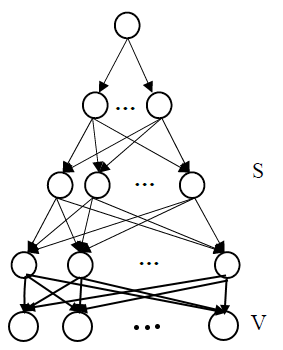
\includegraphics[width= 0.5 \linewidth]{figures/pachinko_dag.png}
	\caption{Illustration of the \gls{dag} structure for the five-level \gls{pam}.}
	\label{fig:pachinko_dag}
\end{figure}

\begin{figure}[h]
	\centering
	\resizebox{0.8\columnwidth}{!}{%
	\begin{tikzpicture}
		[
		observed/.style={minimum size=26pt,circle,draw=blue!50,fill=blue!20},
		unobserved/.style={minimum size=26pt,circle,draw},
		post/.style={->,>=stealth',semithick},
		]
		
		\node (w-j) [observed] at (0,0) {$W$};
		\node (z-4) [unobserved, above of= w-j, node distance=2.5cm] {$Z_{w4}$};
		\node (z-3) [unobserved, left of= z-4, node distance=2cm] {$Z_{w3}$};
		\node (z-2) [unobserved, left of= z-3, node distance=1.5cm] {$Z_{w2}$};
		\node (z-1) [unobserved, left of= z-2, node distance=1.5cm] {$Z_{w1}$};
		
		\node (theta_a) [unobserved, above of= z-2, node distance=2cm] {$\theta_a^d$};
		\node (alpha_a) [unobserved, above of= theta_a , node distance=2cm] {$\alpha_a$};
		
		\node (theta_b) [unobserved, above of= z-3, node distance=2cm] {$\theta_b^d$};
		\node (alpha_b) [unobserved, above of= theta_b , node distance=2cm] {$\alpha_b$};
		
		\node (theta_c) [unobserved, above of= z-4, node distance=2cm] {$\theta_c^d$};
		\node (alpha_c) [unobserved, above of= theta_c , node distance=2cm] {$\alpha_c$};
		
		\node (theta_s2) [unobserved, left of=w-j , node distance=8cm] {$\theta_c$};
		\node (beta) [unobserved, above of=theta_s2 , node distance=2.5cm] {$\beta$};
		
		\path
		(z-4) edge [post] (w-j)
		(z-3) edge [post] (z-4)
		(z-2) edge [post] (z-3)
		(z-1) edge [post] (z-2)
		
		(theta_a) edge [post] (z-2)
		(alpha_a) edge [post] (theta_a)
		
		(theta_b) edge [post] (z-3)
		(alpha_b) edge [post] (theta_b)
		
		(theta_c) edge [post] (z-4)
		(alpha_c) edge [post] (theta_c)
		
		(theta_s2) edge [post] (w-j)
		(beta) edge [post] (theta_s2)
		;
		
		\node [draw,fit=(w-j) (theta_a) (z-1), inner sep=25pt] (plate-context) {};
		\node [above left] at (plate-context.south east) {$N$};
		
		\node [draw,fit=(w-j) (z-1), inner sep=12.5pt] (plate-token) {};
		\node [above left] at (plate-token.south east) {$|d|$};
		
		\node [draw,fit=(theta_s2), inner sep=10pt] (plate-token) {};
		\node [above left] at (plate-token.south east) {$S_3$};
		
		\node [draw,fit=(theta_c) (alpha_c), inner sep=10pt] (plate-token) {};
		\node [above left] at (plate-token.south east) {$S_2$};
		
		\node [draw,fit=(theta_b) (alpha_b), inner sep=10pt] (plate-token) {};
		\node [above left] at (plate-token.south east) {$S_1$};
		
	\end{tikzpicture}}
	\caption{Plate notation for the five-level \gls{pam}.}
	\label{fig:pachinko}
\end{figure}
\vejleder[inline]{a,b,c ~ $t_i$ in Figure 5}
\todo[inline]{make illustrations of dag structur pretty}

\subsubsection{Modification to Pachinko Allocation}
Since only $25\%$ of the documents have an observed taxonomy, we can then lock the words in the observed documents to be in the corresponding topics within the pachinko \gls{dag} instead of continuously sampling them using Gibbs sampling.
This creates some constant context for the topics, which the documents with unobserved taxonomies will be fitted around.

Some of the observed documents have multiple taxonomies.
For these documents, one of the taxonomies is chosen randomly for each word in the document.

\subsection{Combinations}
\todo[inline]{consider the plate notation of combination models}
